\documentclass{article}
\usepackage[utf8]{inputenc}
\usepackage{graphicx}
\usepackage{amsthm}
\usepackage{amsmath}
\usepackage{amssymb}
\usepackage{float}
\usepackage{hyperref}
\usepackage{booktabs}
\usepackage{algorithm2e}
\usepackage{caption}
\usepackage{subcaption}
\usepackage{natbib}



%%%%%%%%%%%%%%%%%%%%%%%%%%%%
% Paper dependent stuff    %
%%%%%%%%%%%%%%%%%%%%%%%%%%%%

\newcommand{\Tau}{T}

\newcommand{\hlrb}[1]{\bm{\textcolor{Red}{#1}}}
\newcommand{\hlbb}[1]{\bm{\textcolor{Blue}{#1}}}
\newcommand{\hlgb}[1]{\bm{\textcolor{Green}{#1}}}

\newcommand{\OPD}{\texttt{OPD}}

%%%%%%%%%%%%%%%%%%%%%%%%%%%%
% Aesthetics               %
% over-underline, hat, bold%
%%%%%%%%%%%%%%%%%%%%%%%%%%%%

\newcommand{\eps}{\varepsilon}
\newcommand{\vareps}{\varepsilon}
\renewcommand{\epsilon}{\varepsilon}
%\renewcommand{\hat}{\widehat}
\renewcommand{\tilde}{\widetilde}
\renewcommand{\bar}{\overline}

\newcommand*{\MyDef}{\mathrm{\tiny def}}
\newcommand*{\eqdefU}{\ensuremath{\mathop{\overset{\MyDef}{=}}}}% Unscaled version
% \newcommand*{\eqdef}{\mathop{\overset{\MyDef}{\resizebox{\widthof{\eqdefU}}{\heightof{=}}{=}}}}
\newcommand{\eqdef}{\stackrel{def}{=}}


\def\:#1{\protect \ifmmode {\mathbf{#1}} \else {\textbf{#1}} \fi}
\newcommand{\CommaBin}{\mathbin{\raisebox{0.5ex}{,}}}

\newcommand{\wt}[1]{\widetilde{#1}}
\newcommand{\wh}[1]{\widehat{#1}}
\newcommand{\wo}[1]{\overline{#1}}
\newcommand{\wb}[1]{\overline{#1}}

% bf and bm missing due to conflict!!
\newcommand{\bsym}[1]{\mathbf{#1}}
\newcommand{\bzero}{\mathbf{0}}
\newcommand{\ba}{\mathbf{a}}
\newcommand{\bb}{\mathbf{b}}
\newcommand{\bc}{\mathbf{c}}
\newcommand{\bd}{\mathbf{d}}
\newcommand{\be}{\mathbf{e}}
\newcommand{\bg}{\mathbf{g}}
\newcommand{\bh}{\mathbf{h}}
\newcommand{\bi}{\mathbf{i}}
\newcommand{\bj}{\mathbf{j}}
\newcommand{\bk}{\mathbf{k}}
\newcommand{\bl}{\mathbf{l}}
\newcommand{\bn}{\mathbf{n}}
\newcommand{\bo}{\mathbf{o}}
\newcommand{\bp}{\mathbf{p}}
\newcommand{\bq}{\mathbf{q}}
\newcommand{\br}{\mathbf{r}}
\newcommand{\bs}{\mathbf{s}}
\newcommand{\bt}{\mathbf{t}}
\newcommand{\bu}{\mathbf{u}}
\newcommand{\bv}{\mathbf{v}}
\newcommand{\bw}{\mathbf{w}}
\newcommand{\bx}{\mathbf{x}}
\newcommand{\by}{\mathbf{y}}
\newcommand{\bz}{\mathbf{z}}

\newcommand{\bA}{\mathbf{A}}
\newcommand{\bB}{\mathbf{B}}
\newcommand{\bC}{\mathbf{C}}
\newcommand{\bD}{\mathbf{D}}
\newcommand{\bE}{\mathbf{E}}
\newcommand{\bF}{\mathbf{F}}
\newcommand{\bG}{\mathbf{G}}
\newcommand{\bH}{\mathbf{H}}
\newcommand{\bI}{\mathbf{I}}
\newcommand{\bJ}{\mathbf{J}}
\newcommand{\bK}{\mathbf{K}}
\newcommand{\bL}{\mathbf{L}}
\newcommand{\bM}{\mathbf{M}}
\newcommand{\bN}{\mathbf{N}}
\newcommand{\bO}{\mathbf{O}}
\newcommand{\bP}{\mathbf{P}}
\newcommand{\bQ}{\mathbf{Q}}
\newcommand{\bR}{\mathbf{R}}
\newcommand{\bS}{\mathbf{S}}
\newcommand{\bT}{\mathbf{T}}
\newcommand{\bU}{\mathbf{U}}
\newcommand{\bV}{\mathbf{V}}
\newcommand{\bW}{\mathbf{W}}
\newcommand{\bX}{\mathbf{X}}
\newcommand{\bY}{\mathbf{Y}}
\newcommand{\bZ}{\mathbf{Z}}

% calligraphic
\newcommand{\cf}{\mathcal{f}}
\newcommand{\cA}{\mathcal{A}}
\newcommand{\cB}{\mathcal{B}}
\newcommand{\cC}{\mathcal{C}}
\newcommand{\cD}{\mathcal{D}}
\newcommand{\cE}{\mathcal{E}}
\newcommand{\cF}{\mathcal{F}}
\newcommand{\cG}{\mathcal{G}}
\newcommand{\cH}{\mathcal{H}}
\newcommand{\cI}{\mathcal{I}}
\newcommand{\cJ}{\mathcal{J}}
\newcommand{\cK}{\mathcal{K}}
\newcommand{\cL}{\mathcal{L}}
\newcommand{\cM}{\mathcal{M}}
\newcommand{\cN}{\mathcal{N}}
\newcommand{\cO}{\mathcal{O}}
\newcommand{\cP}{\mathcal{P}}
\newcommand{\cQ}{\mathcal{Q}}
\newcommand{\cR}{\mathcal{R}}
\newcommand{\cS}{\mathcal{S}}
\newcommand{\cT}{\mathcal{T}}
\newcommand{\cU}{\mathcal{U}}
\newcommand{\cV}{\mathcal{V}}
\newcommand{\cW}{\mathcal{W}}
\newcommand{\cX}{\mathcal{X}}
\newcommand{\cY}{\mathcal{Y}}
\newcommand{\cZ}{\mathcal{Z}}

%%%%%%%%%%%%%%%%%%%%%%%%%%%%
% Math jargon              %
%%%%%%%%%%%%%%%%%%%%%%%%%%%%
\newcommand{\wrt}{w.r.t.\xspace}
\newcommand{\defeq}{\stackrel{\mathclap{\normalfont\mbox{\tiny def}}}{=}}
\newcommand{\maxund}[1]{\max\limits_{#1}}
\newcommand{\supund}[1]{\text{sup}\limits_{#1}}
\newcommand{\minund}[1]{\min\limits_{#1}}
\renewcommand{\epsilon}{\varepsilon}
\newcommand{\bigotime}{\mathcal{O}}


\DeclareMathOperator*{\argmin}{arg\,min} 
\DeclareMathOperator*{\argmax}{arg\,max} 
\DeclareMathOperator*{\cupdot}{\mathbin{\mathaccent\cdot\cup}}

%%%%%%%%%%%%%%%%%%%%%%%%%%%%
% Matrix operators         %
%%%%%%%%%%%%%%%%%%%%%%%%%%%%
\newcommand{\transpose}{^\mathsf{\scriptscriptstyle T}}
\newcommand{\transp}{\mathsf{\scriptscriptstyle T}}

%%%%%%%%%%%%%%%%%%%%%%%%%%%%
% Statistic operators      %
%%%%%%%%%%%%%%%%%%%%%%%%%%%%
\newcommand{\probability}[1]{\mathbb{P}\left(#1\right)}
\newcommand{\probdist}{Pr}
\DeclareMathOperator*{\expectedvalue}{\mathbb{E}}
\DeclareMathOperator*{\variance}{\text{Var}}
\newcommand{\expectedvalueover}[1]{\expectedvalue\limits_{#1}}
\newcommand{\condbar}{\;\middle|\;}
\newcommand{\gaussdistr}{\mathcal{N}}
\newcommand{\uniformdistr}{\mathcal{U}}
\newcommand{\bernoullidist}{\mathcal{B}}

%%%%%%%%%%%%%%%%%%%%%%%%%%%%
% Algebraic Sets           %
%%%%%%%%%%%%%%%%%%%%%%%%%%%%
\newcommand{\Real}{\mathbb{R}}
\newcommand{\Natural}{\mathbb{N}}
\newcommand{\statespace}{\mathcal{X}}
\newcommand{\funcspace}{\mathcal{F}}
\newcommand{\dynaspace}{\mathcal{T}}

%
%\newtheorem{theorem}{Theorem}
%\newtheorem{definition}{Definition}
%\newtheorem{lemma}{Lemma}
%\providecommand*\lemmaautorefname{Lemma}
%\newtheorem{proposition}{Proposition}
%\providecommand*\propositionautorefname{Proposition}
%\newtheorem{remark}{Remark}
%\newtheorem{property}{Property}
%\newtheorem{assumption}{Assumption}
%\providecommand*\assumptionautorefname{Assumption}
%\newtheorem{conjecture}{Conjecture}
\providecommand*\algorithmautorefname{Algorithm}

\addto\extrasenglish{  
	\def\algorithmautorefname{Algorithm}  
}
%
%\newtheorem*{definition*}{Definition}
%\newtheorem*{theorem*}{Theorem}
%\newtheorem*{proposition*}{Proposition}
%\newtheorem*{remark*}{Remark}

\title{Planning with States}
\author{Edouard Leurent}
\date{October 2019}

\begin{document}

\maketitle

\tableofcontents

\section{Motivation}

Traditional planning algorithms sample sequences of actions by considering sequences of rewards only. Can we leverage state information during planning, to account for the fact that different sequences can lead to similar states, and hence similar future rewards?

\section{Deterministic Systems with Discrete States}

We consider an MDP with discrete state space and deterministic dynamics.

\begin{paragraph}{Notations}
We denote:
\begin{itemize}
\item $n$ the number of expanded nodes, $\Tau_n$ the tree obtained after $n$ node expansions, and $\cL_n$ the set of its leaves.
    \item $s(a)$ the state reached after running sequence $a$, and $\cN_n(a)$ the set of \emph{neighbours} of $a$, that lead to the same state:  \[\cN_n(a) = \{a'\in\Tau_n: s(a)=s(a')\}\]
\end{itemize}
\end{paragraph}

\begin{definition}[Values]
The value of a \textbf{state} $s\in S$ is:
\begin{equation}
    V(s) = \max_{a\in A^\infty} \sum_{t=0}^\infty \gamma^t r(a_{1:t}),\, \text{starting from the state $s$,}
\end{equation}




and the value of a \textbf{sequence} of actions $a\in A^h$ is:
\begin{equation}
\label{eq:state_value}
    V(a) = \sum_{t=0}^{h-1} \gamma^t r(a_{1:t}) + \gamma^{h} V(s(a)),\, \text{starting from $s_0$.}
\end{equation}
\end{definition}

\begin{definition}[Upper confidence bounds]

We denote by $U:\Tau_n \rightarrow \Real$ an upper-bound for the state-value $V(s(a))$ that verifies:
\begin{equation*}
    \forall a\in\Tau_n, \qquad V(s(a)) \leq U(a)
\end{equation*}

For instance, since assume that the rewards are bounded in [0, 1], a trivial upper-bound on $V(s(a))$ is:
\[V(s(a)) \leq V_{\max} = \frac{1}{1-\gamma} \]

The state-value bound $U$ induces an upper-bound $B(U)$ for sequences values defined as:
\begin{equation}
\label{eq:sequence_value}
    V(a) \leq B(U)(a) \eqdef \sum_{t=0}^{h-1} \gamma^t r(a_{1:t}) + \gamma^{h} U(a)
\end{equation}
\end{definition}

This provides an optimistic sampling rule for sequences of actions:
\begin{equation}
    \label{eq:sampling_rule}
    a_{n+1} = \argmax_{a\in\cL_n} B(U)(a)
\end{equation}
Our goal is to make this bound $U$ as tight as possible given available information.

\begin{definition}[Bellman Optimal operator]
We define the Bellman Optimal operator $L$ over $\Real^{\Tau_n}$ as:

\begin{equation}
    L(U)(a) = \begin{cases}
    U(a) & \text{if $a\in\mathcal{L}_n$;} \\
    \min(U(a), \max_{b\in A} r(ab) + \gamma L(U)({ab}))
    & \text{else.}
    \end{cases}
\end{equation}

Note that a $\min$ was added to the traditional Bellman backup in order to maintain the upper-bound of a node if it is already  tighter than the backup of its children.

It is easily seen that $L^2=L$ and:
\begin{equation*}
    V \leq U \implies V \leq L(U) \leq U
\end{equation*}

\end{definition}

In \texttt{OPD}, they used the following bound over sequences: $B\left(L\left(V_{\max}\right)\right)$.

\section{Tree-based State-aware planning}

We extend \texttt{OPD} to include the two following ideas:

\subsection{Aggregation of state values}
\label{sec:aggregation}

Let $U\in\Real^{\Tau_n}$ a state-value upper-bound.

\begin{definition}[Aggregation operator]
If several sequences $a'\in\Tau_n$ lead to the same state $s$, their upper-bounds must all hold. This defines an aggregation operator $A$ over functions in $\Real^{\Tau_n}$ as:
    \begin{equation}
    \label{eq:aggregation}
        \forall a\in\mathcal{T}_n, \quad A(U)(a) = \min_{a'\in \cN_n(a)} U(a'),
    \end{equation}
    
Again, we have $A^2=A$ and:
\begin{equation*}
    V \leq U \implies V \leq A(U) \leq U
\end{equation*}
\end{definition}

At this stage, we have defined two operators $A$ and $L$ that operate on UCBs $U$ and can only tighten them. It is natural to try and apply both of them until convergence: $U = A(U) = L(U)$.


\begin{remark}[Interplay of backups and aggregations]
We can notice that the sampling rule \eqref{eq:sampling_rule} only depends on the value of $U$ at the leaves $\cL_n$. Hence, it seems that:
\begin{itemize}
    \item applying $L$ alone is not useful, since information only travels upwards in the tree $\Tau_n$;
    \item conversely, applying $A$ can update the value of any node in the tree $\Tau_n$, including leaves $\cL_n$.
\end{itemize}
Hence, the aggregation $A$ makes the backup $L$ useful: each $L$ backup can provide tighter bounds $U(s')$ for states $s'$ at inner-nodes which can in turn be aggregated with $A$ and propagated down in the tree, potentially affecting the leaves and future exploration. 
\end{remark}

This suggests an alternating procedure of state-aggregations $A$ and Bellman-backups $L$, whose convergence, sample complexity and efficiency must be studied.

\begin{proposition}[Contractivity of $AL$]
$A$ is a 1-Lipschitz operator, which makes $AL$ a $\gamma$-contraction.
\end{proposition}
\begin{proof}
Let $U_1, U_2\in \Real^\Tau_n, a\in\Tau_n$,
\begin{align*}
    (AU_1 - AU_2)(a) &= \min_{a'\in\cN_n(a)} U_1(a') - \min_{a'\in\cN_n(a)} U_2(a') \\
    &= \min_{a'\in\cN_n(a)} U_1(a') - U_2(a^-) \\
    &\leq U_1(a^-) - U_2(a^-) \\
    &\leq \|U_1 - U_2\|_\infty
\end{align*}
where $a^-\in \argmin_{a'\in\cN_n(a)} U_2(a')$. 
Hence, $\|AU_1 - AU_2\|_\infty \leq \|U_1 - U_2\|_\infty$
\end{proof}

We can perform fixed-point iteration of alternating backups and aggregations starting from the trivial state-value $U_0 = V_{\max}$.

\begin{equation}
    \label{eq:recursion}
    U_k = (AL)^k(V_{\max})
\end{equation}
$(U_k)$ is decreasing and converges at a rate $\gamma^k$, but it will not converge in finite time whenever there is a loop, as shown in \autoref{fig:simple_loop}. We can decide to stop whenever a desired accuracy is reached: 

\begin{proposition}[Early stopping]
If we have that
\[\forall a\in\Tau_n, |U_{k+1}(a) - U_k(a)| \leq \epsilon (1-\gamma)\gamma^{-h(a)-1},\]
then the sequence value $B(U_{\infty})$ is approximated with an accuracy of $\epsilon$.
\end{proposition}
\begin{proof}
Let $a\in A^h$. We consider the sequence $(B(U_n))_{n\in\Natural}$.
Notice that for any $U,V\in\Real^\Tau$, we have $B(U)(a)-B(V)(a)=\gamma^h(U(a)-V(a))$.

Hence, if the premise holds,
\begin{align*}
    |B(U_{k+1})(a) - B(U_{k})(a)| &\leq \gamma^h\epsilon (1-\gamma)\gamma^{-h-1} = \epsilon (1-\gamma)\gamma^{-1}
\end{align*}

And then, 
\begin{align*}
|B(U_{k+1})(a) - B(U_\infty)(a)| &= \gamma^h |U_{k+1}(a) - U_\infty(a)|\\
&\leq \gamma^{h+1}|U_{k}(a) - U_\infty(a)| \text{ since $LA$ is a $\gamma$-contraction}\\
&\leq \gamma^{h+1}|U_{k}(a) - U_{k+1}(a)| + \gamma^{h+1}|U_{k+1}(a) - U_\infty(a)|\\
&= \gamma|B(U_{k})(a) - B(U_{k+1})(a)| + \gamma |B(U_{k+1})(a) - B(U_\infty)(a)|\\
&\leq \frac{1}{1-\gamma}\gamma |B(U_{k})(a) - B(U_{k+1})(a)|\\
&\leq\epsilon
\end{align*}

\end{proof}

\begin{figure}
    \centering
    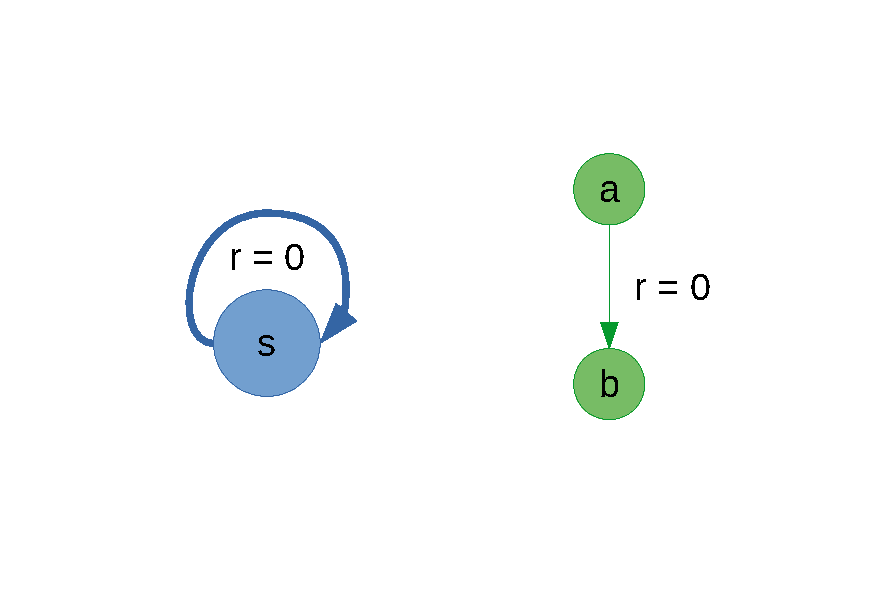
\includegraphics[trim=2cm 2cm 2cm 2cm, clip, width=0.4\textwidth]{img/simple_loop.pdf}\\
    \begin{tabular}{cccccc}
         \toprule
         & $U_0$ & $L (U_0)$ & $AL(U_0)$ & $\cdots$ & $U_k$ \\
         \midrule
         $a$ & $V_{\max}$ & $\gamma V_{\max}$ & $\gamma V_{\max}$ && $\gamma^k V_{\max}$\\
         $b$ & $V_{\max}$ & $V_{\max}$ & $\gamma V_{\max}$ && $\gamma^k V_{\max}$\\
         \bottomrule
    \end{tabular}
    \caption{\textbf{Top}: a looping MDP with $|S|=|A|=1$, and the corresponding expanded tree $\Tau_1$ for a single observed transition. \textbf{Bottom}: the sequence of upper-bounds $(U_n)$ when alternating $A$ and $L$. We obtain $U_k = \gamma^k V_{\max}$ that only goes to $0$ geometrically.}
    \label{fig:simple_loop}
\end{figure}

Alternatively, we can stop after a fixed number of iterations, e.g. $k=2$.

\subsection{Leaves pruning}
\label{sec:pruning}

Another observation can be made in the case where two nodes $a_1,a_2\in\Tau_n$ lead to the same state $s$:
\begin{proposition}[Pruning rule]
\label{prop:pruning}
Let $a_1,a_2\in\Tau_n$ such that state $s(a_1) = s(a_2) = s$ and $U = A(U) \geq V$ an aggregated upper-bound. 
\begin{equation}
\label{eq:pruning}
    \text{If } h(a_2) \geq h(a_1) \text{ and } B(U)(a_2) \geq B(U)(a_1)
    \text{, then }V(a_2) \geq V(a_1)
\end{equation}

In particular, there is no need to ever expand the node $a_1$.
\end{proposition}
\begin{proof}
Assume $h(a_2) \geq h(a_1)$.
\begin{align*}
    V(a_1) - V(a_2) &= R(a_1)- R(a_2) + \underbrace{\left(\gamma^{h(a_1)} - \gamma^{h(a_2)}\right)}_{\geq 0}V(s) \\
    &\leq R(a_1)- R(a_2) + \left(\gamma^{h(a_1)} - \gamma^{h(a_2)}\right)U(s)\\
    &= B(U)(a_1) - B(U)(a_2)
\end{align*}
Hence, if this last term is negative, then $V(a_1) - V(a_2)$ is as well.
\end{proof}

We propose that at each step, we detect such pairs $a_1, a_2$. Whenever $a_1$ is a leaf, we can remove it from the set $\cL_n^-\subset \cL_n $ of candidates for expansion.

\section{Regret bound}

\paragraph{Near-optimality}

We define the branching factor $\kappa(U)\in[1, K]$ of near-optimal nodes \emph{according to a state-value bound $U$} as:
\begin{equation}
    \kappa(U) \eqdef \limsup_{h\rightarrow\infty} \left|\left\{a\in A^h: V^* - V(a)\leq \gamma^{h}U(s(a))\right\}\right|^{1/h}.
\end{equation}
This branching factor shrinks as the bound $U$ gets tighter:
\begin{lemma}
If $U_1$ is a tighter bound that $U_2$, its corresponding effective branching factor is lower:
\[U_1\leq U_2\implies \kappa(U_1) \leq \kappa(U_2).\]
\end{lemma}


\begin{theorem}
If $U$ is a valid upper-bound on the state-value $V\leq U$, then optimistic planning with $B(U)$ gives the following simple regret bound: %$\forall \kappa>\kappa(U)$,
\begin{align*}
V^* - V({a_n}) = \cO\left(n^{-\frac{\log 1/\gamma}{\log \kappa(U)}}\right);
\end{align*}
\end{theorem}

And in particular, planning with $U=U_\infty$ gives a potentially better bound $\kappa(U_\infty)$ than planning with $U=V_{\max}$ as in \texttt{OPD}.

\begin{proof}
	As in \citep[][Theorem 2]{Hren2008}, we first show that the simple regret $r_n$ is bounded by $\frac{\gamma^{d_n}}{1 - \gamma}$ where $d_n$ is the depth of $\mathcal{T}_n$. This properties relies on the fact that the returned action belongs to the deepest explored branch, which we can show likewise by contradiction: if there exist some node $i$ of depth $d_n$ and $j$ of depth $d<d_n$ such that $L_j(n) < L_i(n)$, there exists a time $t<n$ where node $i$ was expanded, which means $B(U)_i(t) \geq B(U)_j(t)$. But this is impossible since $B(U)_i(t) = L_i(t) + \gamma^d_n U_i(n) \leq L_i(n) + \gamma^{d_n} U_i(n) < L_j(n) + \gamma^d U_j(n) = B(U)_j(n) \leq B(U)_j(t)$.
	
	This yields directly that the returned action $a = i_0$ where $i$ is some node of maximal depth $d_n$ expanded at round $t\leq n$, which by selection rule verifies $B_a(t) = B_i(t) = \max_{x\in\mathcal{A}} B_x(t)$ and:
	\begin{align*}
	\label{eq:Rndn}
	V - V_a = V_{a^{\star}} - V_a  \leq B_{a^{\star}}(t) - V_a &\leq B_{a}(t) - U_a(t) \\
	&= B_{i}(t) - U_i(t) \\
	&= \frac{\gamma^{d_n}}{1-\gamma}.
	\end{align*}
	
	Secondly, they bound the depth $d_n$ of $\mathcal{T}_n$ with respect to $K$. To that end, they show that the expanded nodes always belong to the sub-tree $\mathcal{T}_\infty$ of all the nodes of depth $d$ that are $\frac{\gamma^d}{1-\gamma}$-optimal. Indeed, if a node $i$ of depth $d$ is expanded at round $k$, then $B_i(t) \geq B_j(t)$ for all $j\in \mathcal{L}_n$ by selection rule, thus the max-backups of \eqref{eq:robust-b-values} up to the root yield $B^r_i(t) = B_\emptyset(t)$. Moreover, by Lemma \ref{lemma:uvb} we have that $B_\emptyset(t) \geq V_\emptyset = V$ and so $V_i \geq U_i(t) = B_i(t) - \frac{\gamma^d}{1-\gamma} \geq V - \frac{\gamma^d}{1-\gamma}$, thus $i \in \mathcal{T}_\infty$.
	
	Then from the definition of $\kappa$ applied to nodes in $\mathcal{T}_\infty$, there exists $d_0$ and $c$ such that the number $n_d$ of nodes of depth $d \geq d_0$ in $\mathcal{T}_\infty$ is bounded by $c\kappa^d$. As a consequence, 
	\begin{eqnarray*}
		K &= \sum_{d=0}^{d_n} n_d = n_0 + \sum_{d=d_0+1}^{d_n} n_d \leq n_0 + c\sum_{d={d_0+1}}^{d_n} \kappa^d.
	\end{eqnarray*}
	
	\begin{itemize}
		\item If $\kappa > 1$, then $K \leq n_0 + c\kappa^{d_0+1}\frac{\kappa^{d_n-d_0}-1}{\kappa-1}$ and thus $d_n \geq d_0 + \log_\kappa \frac{(K-n_0)(\kappa - 1)}{c\kappa^{d_0+1}}$.
		
		We conclude that $r_n \leq \frac{\gamma^{d_n}}{1-\gamma} = \frac{1}{1-\gamma} \left( \frac{(K-n_0)(\kappa - 1)}{c\kappa^{d_0+1}} \right)^\frac{\log \gamma}{\log \kappa} = \cO\left(K^{-\frac{\log 1/\gamma}{\log \kappa}}\right)$.
		
		\item If $\kappa = 1$, then $K \leq n_0 + c(d_n-d_0)$, hence we have $r_n = O\left(\gamma^{Kc}\right)$.
	\end{itemize}
\end{proof}

\section{Efficient implementation}

\paragraph{Time complexity}
 At each step, we perform a value iteration on $n$ nodes, which takes about $\cO\left(\frac{n K}{\log 1/\gamma}\right)$ steps. The entire planning procedure is $\cO\left(\frac{n^2 K}{\log 1/\gamma}\right)$.

In this section, we consider more efficient ways to implement the aggregation/backup and pruning rules described respectively in sections \ref{sec:aggregation} and \ref{sec:pruning}.

\paragraph{Aggregation and backup}
Let us denote $U^{(n)}$ the upper-bound used in the sampling rule \eqref{eq:sampling_rule} after $n$ leaf expansions, where $U^{(n)}$ is defined as the limit of \eqref{eq:recursion}. Assume that the previous iteration $n$, we stopped at some equilibrium $U^{(n)} = L(U^{(n)}) = A(U^{(n)})$.

At step $n+1$, after leaf expansion we obtain a novel tree $\Tau_{n+1}$. Instead of recomputing $U^{(n+1)}$ entirely from scratch using \eqref{eq:recursion}, we can instead initialise it with the previous value $U^{(n)}$ on $\Tau_n$ and $V_{\max}$ on the newly created leaves in $\Tau_{n+1} \setminus \Tau_n$.

We can notice that if we change the value of a single node $a$, the application of $L$ will only modify $U^{(n)}$ at its parents and leave the rest of the tree unchanged. Likewise, applying $A$ will only modify the values for the nodes in $\cN_n(a)$ and leave the rest of the tree unchanged. The idea of \autoref{algo:efficient} is

\paragraph{Leaves pruning}

When and how should we apply the rule \eqref{eq:pruning} described in Proposition \autoref{prop:pruning}?

The most straightforward way is to apply it once at every step, after the aggregations and backups.
The procedure needs to be applied within some equivalence classes $C(a)$ of nodes $a'$ that lead to the same state $s(a')=s(a)$. If a class $C$ is of size $n_C$, then the cost of running \eqref{eq:pruning} is $\cO(n_C^2)$. This could be improved to $\cO(n_C \log n_C)$ by computing the convex hull of the candidates points in $C$. Indeed, any point $a_1$ that does not belong to the top-frontier of this hull is dominated by some $a_2$, in the sense of \eqref{eq:pruning}.


\begin{algorithm}[htp]
  \SetAlgoLined\DontPrintSemicolon
  \SetKwFunction{expand}{expand}
  \SetKwFunction{update}{update}
  \SetKwFunction{backup}{backup}
  \SetKwProg{myalg}{Algorithm}{}{}
  \myalg{\expand{a}}{
  \For{action $b\in A$}{
  \nl Simulate action $b$ from state $s(a)$, observe reward $r$ and next state $s'$\;
  \nl Create a new node $ab$ with reward $r$,  state $s'$\;
  }
  \nl \update{a}\;
  \;
  }
  
  \setcounter{AlgoLine}{0}
  \SetKwProg{myproc}{Procedure}{}{}
  \myproc{\update{a}}{
  \uIf{$a$ is not a leaf}{
      \nl $U_{\text{backup}} \leftarrow \max_{b\in A} r(ab)+ \gamma U(s(ab))$\tcp*{Bellman backup $L$}
      \nl $\Delta \leftarrow U(s(a)) -  U_{\text{backup}}$\tcp*{Is the new bound tighter?}
      \nl \lIf{$\Delta > 0$}{$U(s(a))\leftarrow U_{\text{backup}}$\tcp*{Aggregation $A$}}
      \For{$a'\in\cN_n(a)$\tcp*{Recursion over updated nodes}}{
          \uIf{$a'$ is not the root and $\Delta > \epsilon(1-\gamma)\gamma^{-h(a)}$}{
              \nl \update{parent of $a'$}
          }
          }
  }
  }
  \caption{An recursive implementation of $(LA)^\infty$ with leaves pruning}
  \label{algo:efficient}
\end{algorithm} 

\section{Experiments}

\subsection{Full algorithm}

\subsubsection{Two-armed bandit}

We consider the simplest possible problem: 1 state and 2 actions, with rewards 0 and 1. The state-aware planner never expands a suboptimal node. In contrast, the tree expanded by \texttt{OPD} is quite balanced, even with such a dense reward and important gap.
\begin{figure}[H]
    \centering
    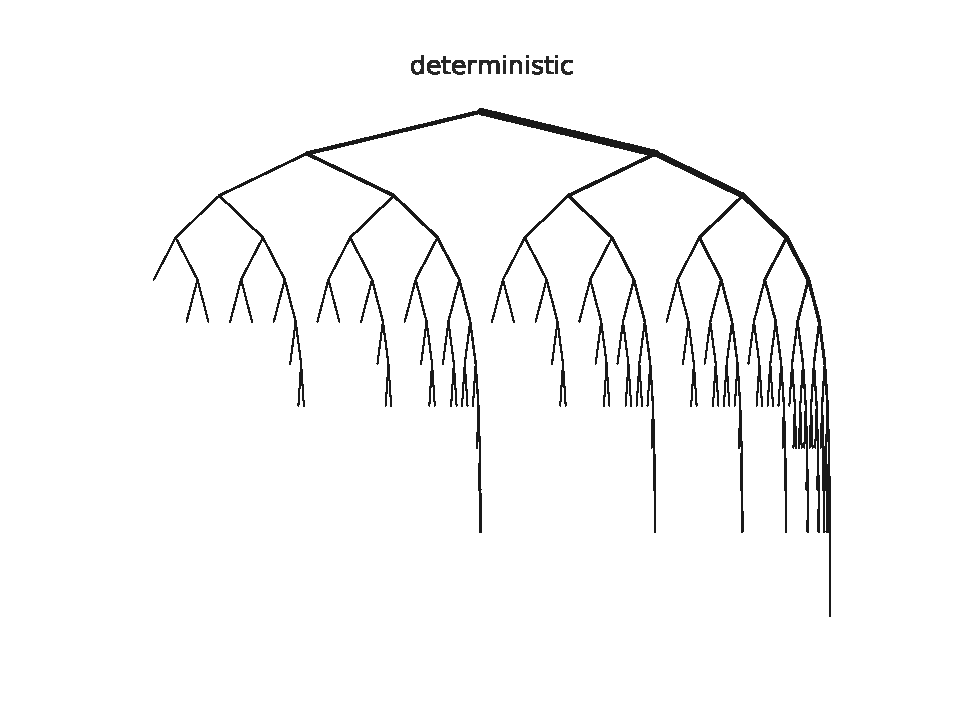
\includegraphics[width=0.49\textwidth]{img/bandit_deterministic.pdf}
    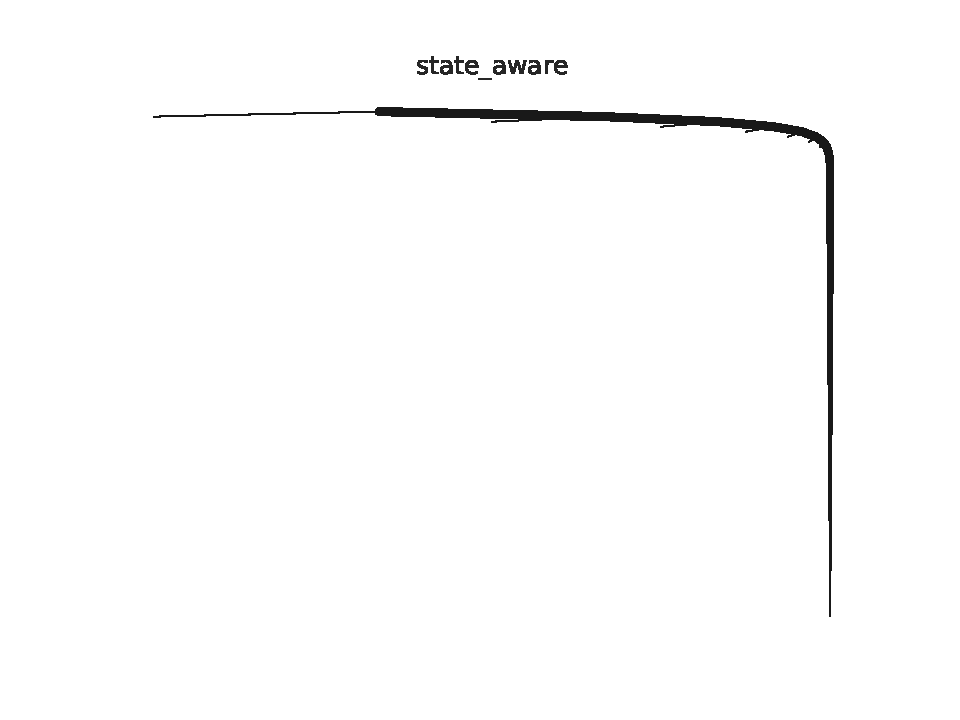
\includegraphics[width=0.49\textwidth]{img/bandit_state_aware.pdf}
    \caption{Trees expanded for $n = 200$, $\gamma=0.99$}
    \label{fig:bandit_trees}
\end{figure}

\subsubsection{Gridworld with 4 actions}

The reward is a paraboloid centred at $(10, 10)$ with length-scale of 5:  $r(x, y) = 1 - \frac{1}{5^2}((x-10)^2 + (y-10)^2)$ clipped to [0, 1].

\begin{figure}[H]
    \centering
    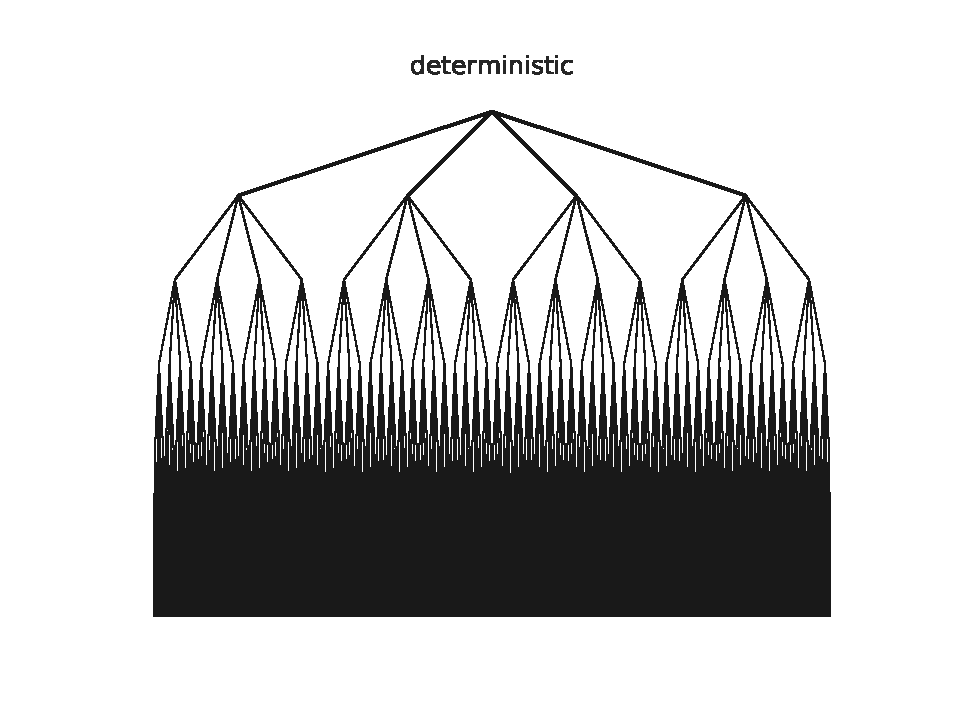
\includegraphics[width=0.49\textwidth]{img/4_deterministic.pdf}
    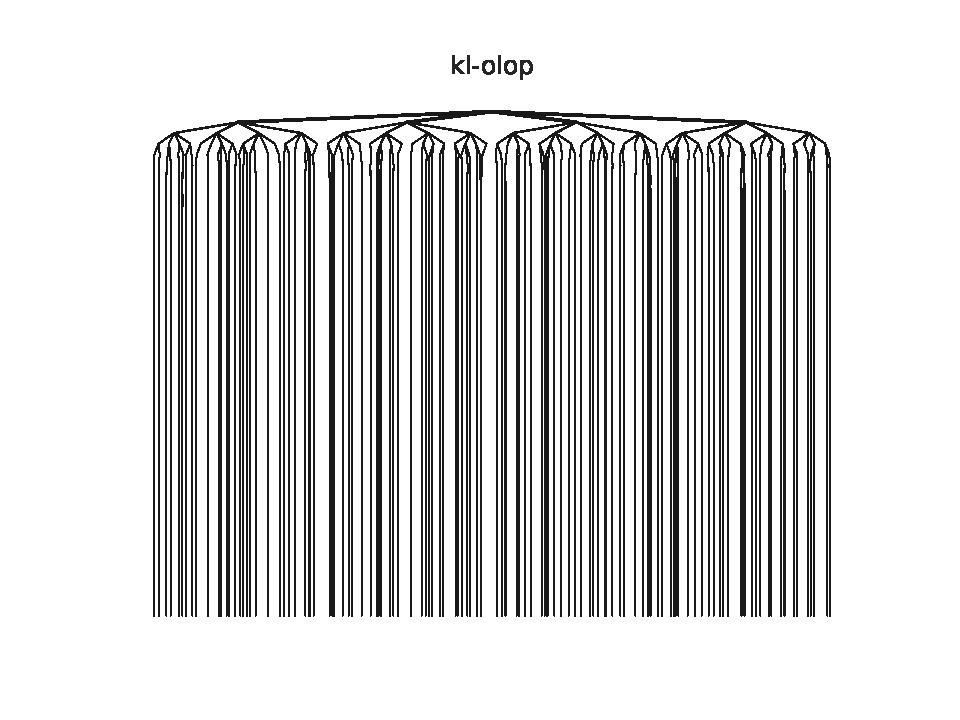
\includegraphics[width=0.49\textwidth]{img/4_kl-olop.pdf}
    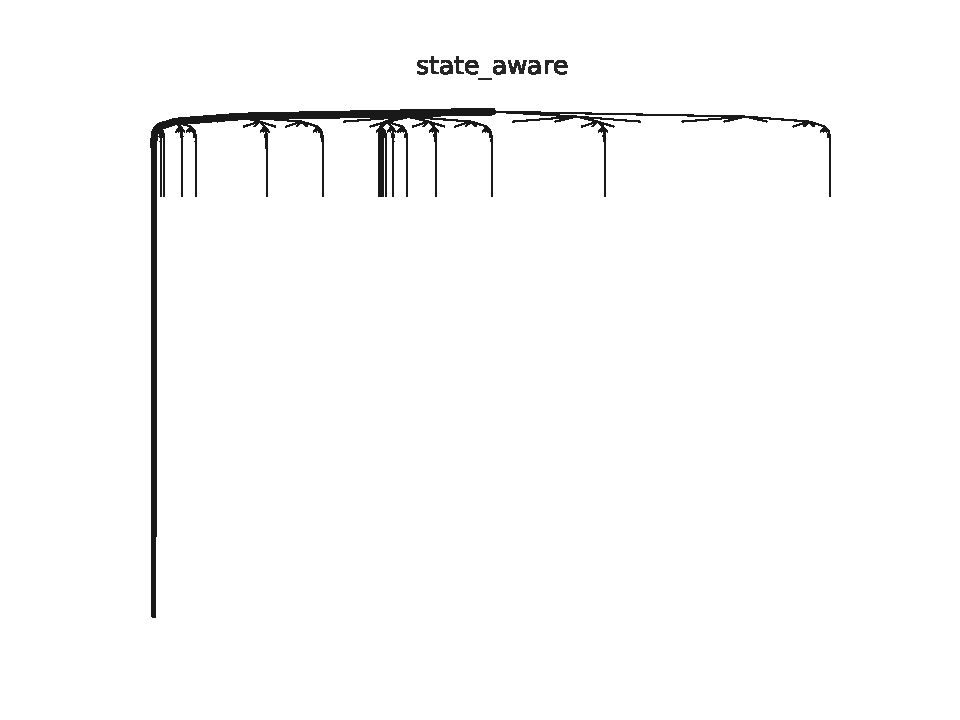
\includegraphics[width=0.49\textwidth]{img/4_state_aware.pdf}
    \caption{Trees expanded for $n = 5460$, $\gamma=0.95$}
    \label{fig:gw4_trees}
\end{figure}
\begin{figure}[H]
    \centering
    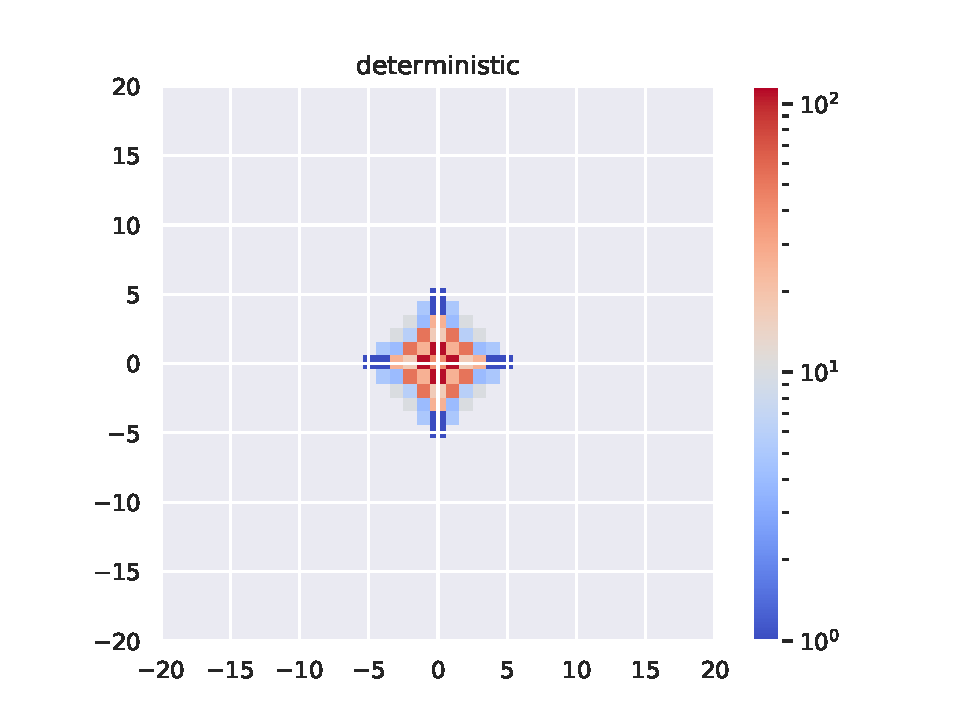
\includegraphics[width=0.49\textwidth]{img/4_occupations_deterministic.pdf}
    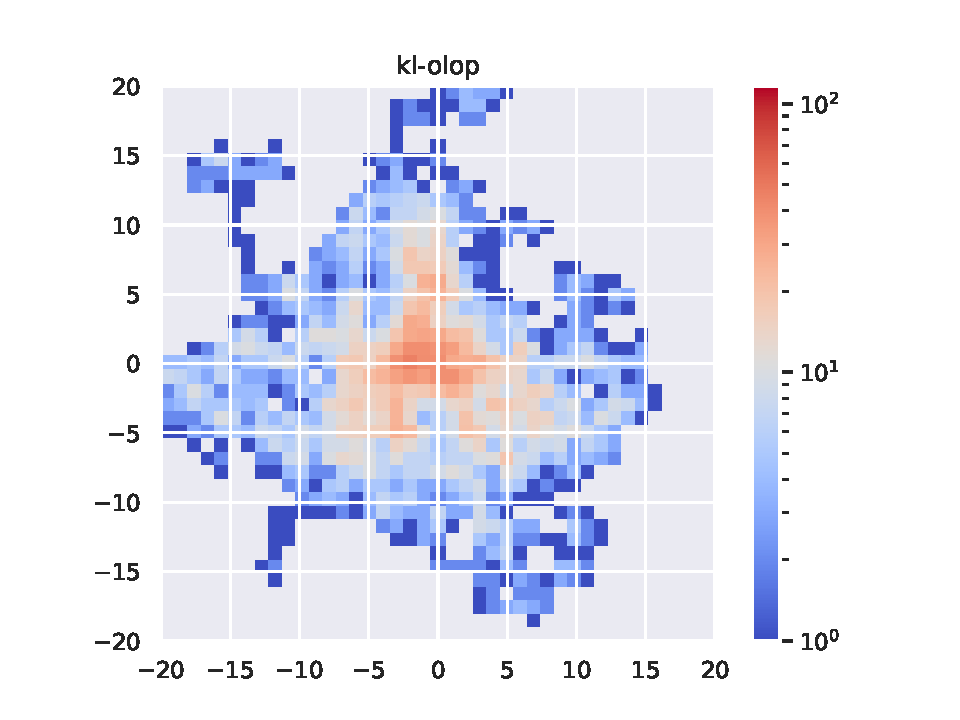
\includegraphics[width=0.49\textwidth]{img/4_occupations_kl-olop.pdf}
    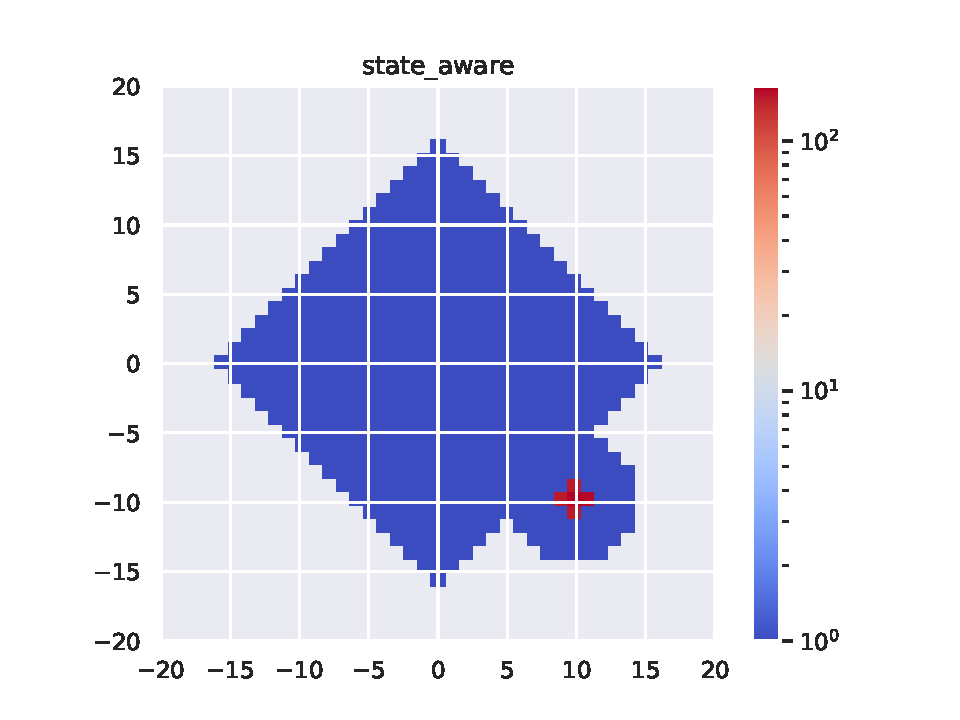
\includegraphics[width=0.49\textwidth]{img/4_occupations_state_aware.pdf}
    \caption{Number of visits for $n = 5460$, $\gamma=0.95$}
    \label{fig:gw4_visits}
\end{figure}
\begin{figure}[H]
    \centering
    % \includegraphics[width=0.49\textwidth]{img/4_updates_deterministic.pdf}
    % \includegraphics[width=0.49\textwidth]{img/4_updates_kl-olop.pdf}
    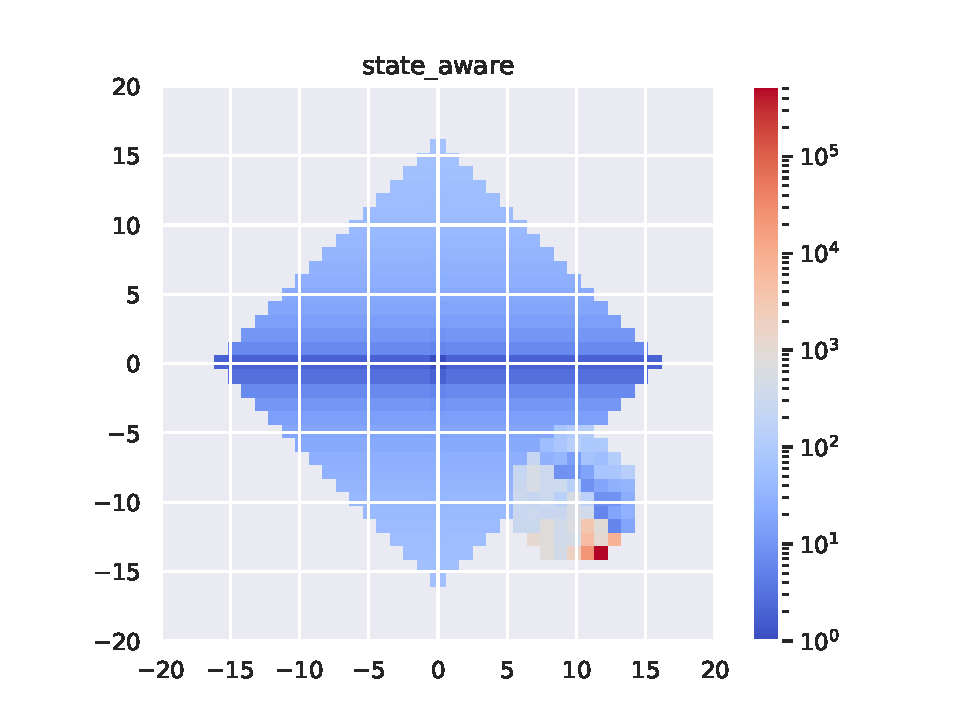
\includegraphics[width=0.49\textwidth]{img/4_updates_state_aware.pdf}
    \caption{Number of updates in the leaf expansion for $n = 5460$, $\gamma=0.95$}
    \label{fig:gw4_updates}
\end{figure}

% \subsubsection{Gridworld with 8 actions}

% We add the diagonal actions.

% \begin{figure}[H]
%     \centering
%     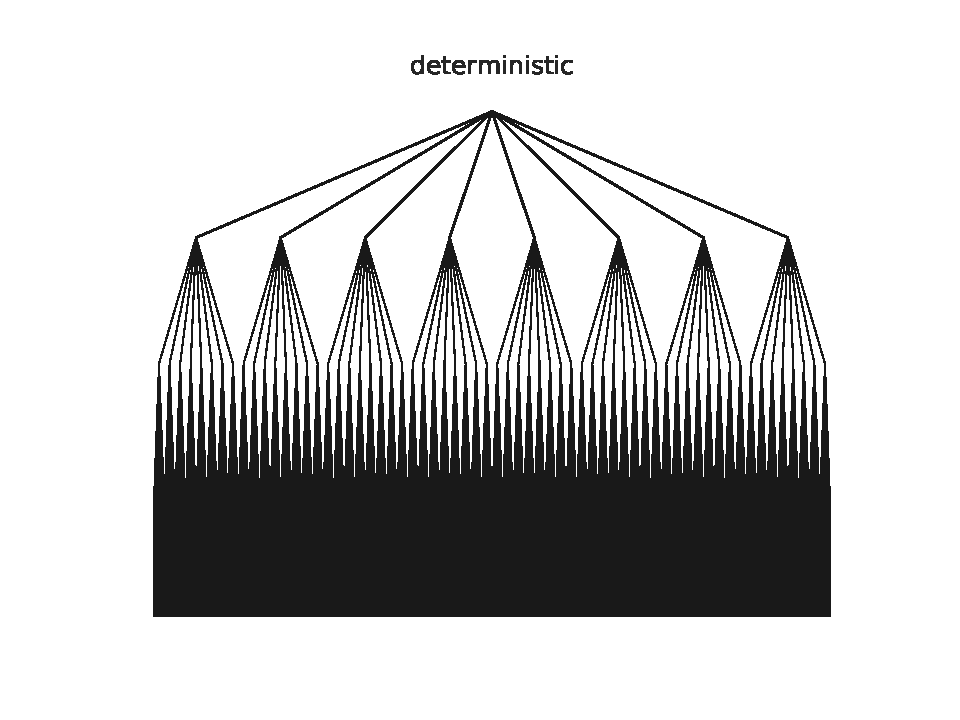
\includegraphics[width=0.49\textwidth]{img/8_deterministic.pdf}
%     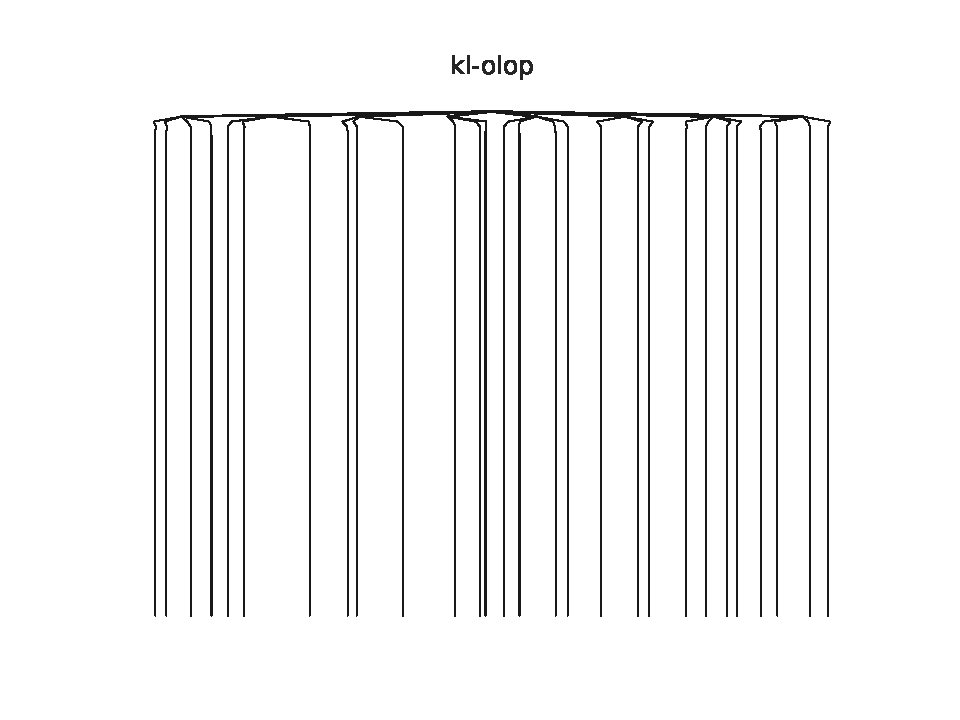
\includegraphics[width=0.49\textwidth]{img/8_kl-olop.pdf}
%     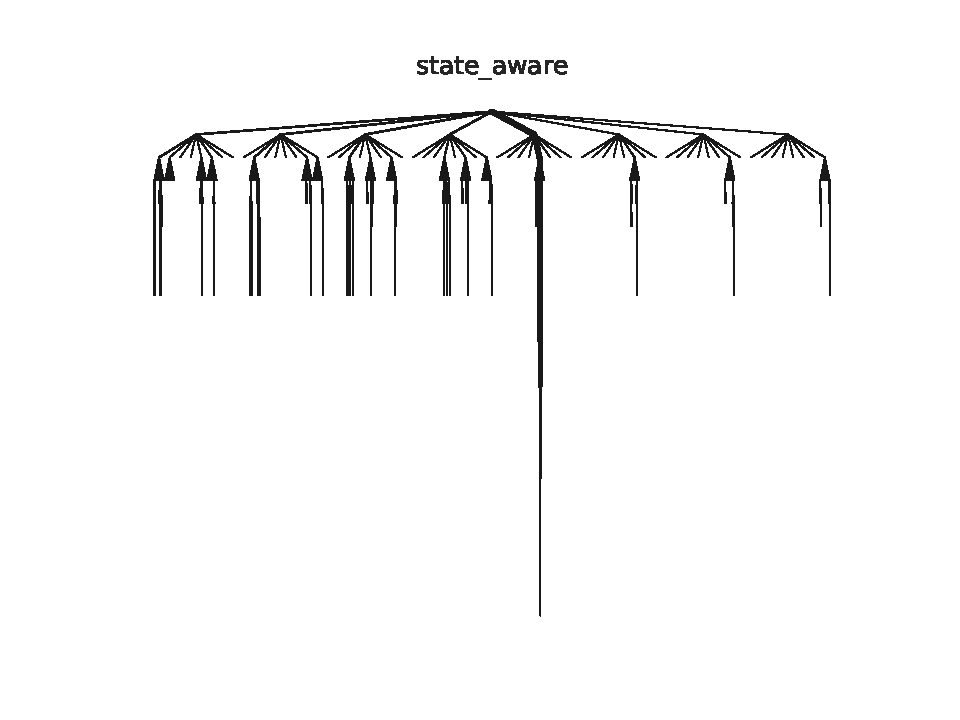
\includegraphics[width=0.49\textwidth]{img/8_state_aware.pdf}
%     \caption{Trees expanded for $n = 4680$, $\gamma=0.95$}
%     \label{fig:my_label}
% \end{figure}
% \begin{figure}[H]
%     \centering
%     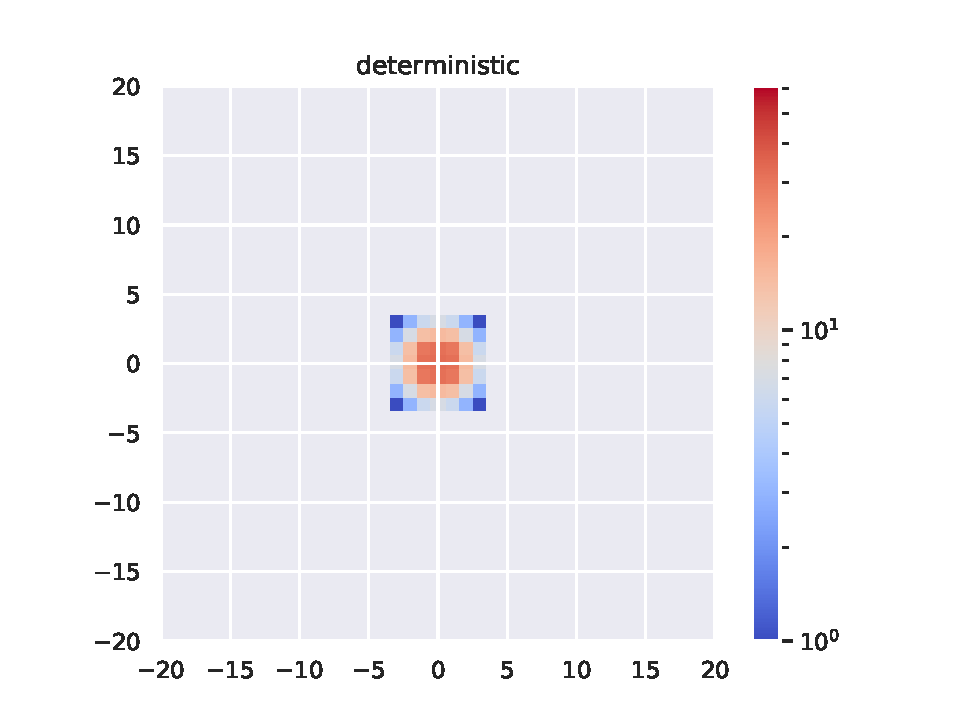
\includegraphics[width=0.49\textwidth]{img/8_states_deterministic.pdf}
%     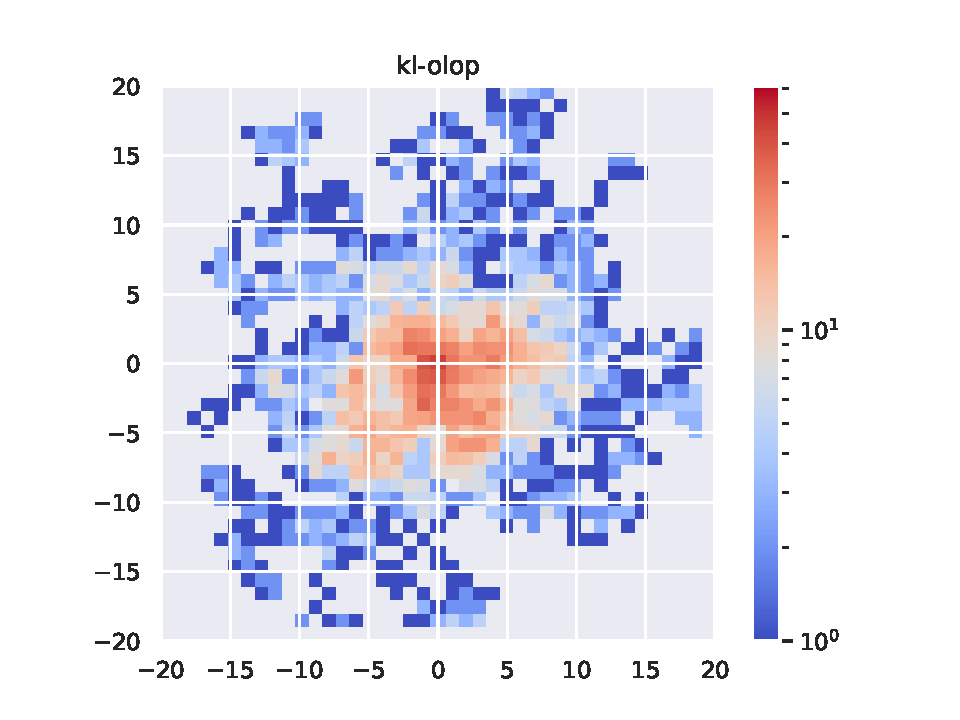
\includegraphics[width=0.49\textwidth]{img/8_states_kl-olop.pdf}
%     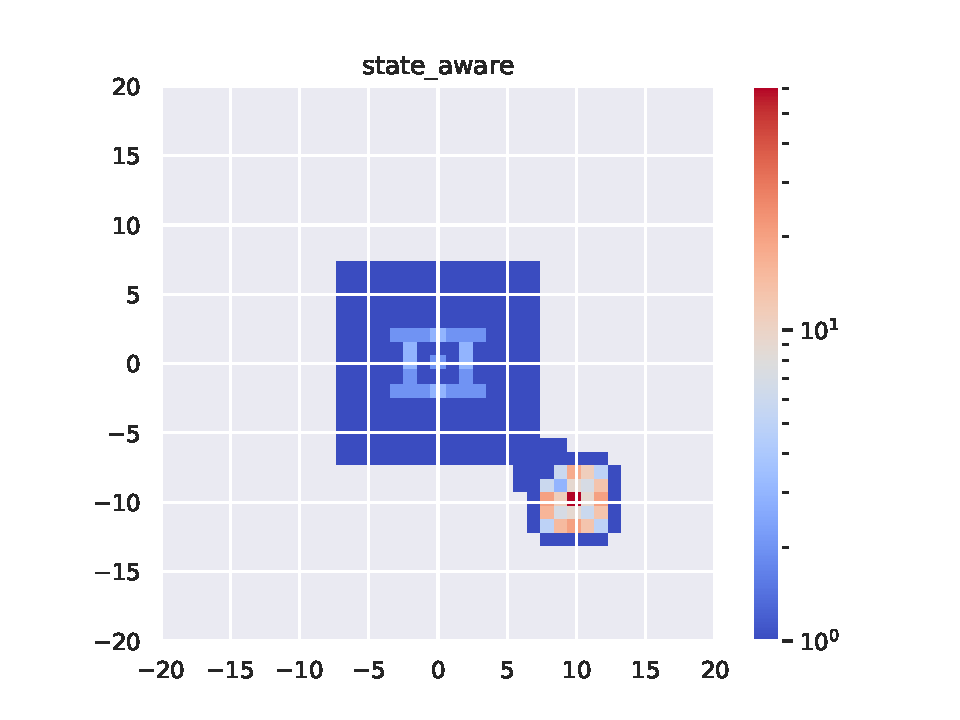
\includegraphics[width=0.49\textwidth]{img/8_states_state_aware.pdf}
%     \caption{Trees expanded for $n = 4680$, $\gamma=0.95$}
%     \label{fig:my_label}
% \end{figure}

\subsection{Effect of the early stopping}

\begin{figure}[H]
    \centering
    \begin{subfigure}[b]{\textwidth}
        \centering
        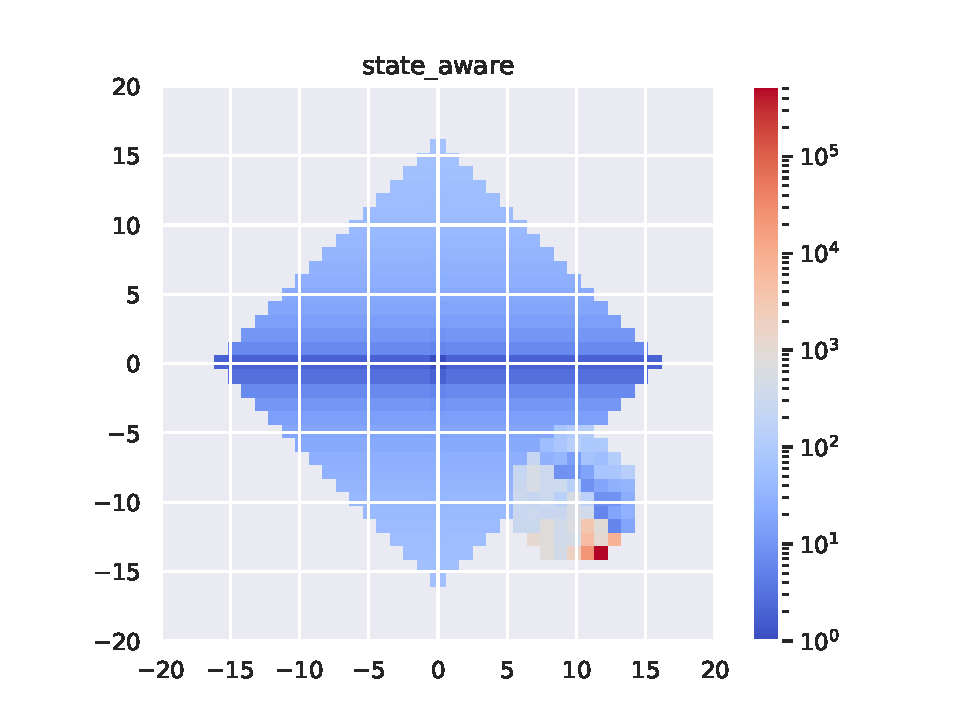
\includegraphics[width=0.49\linewidth]{img/epsilon/0/updates_state_aware.pdf}
        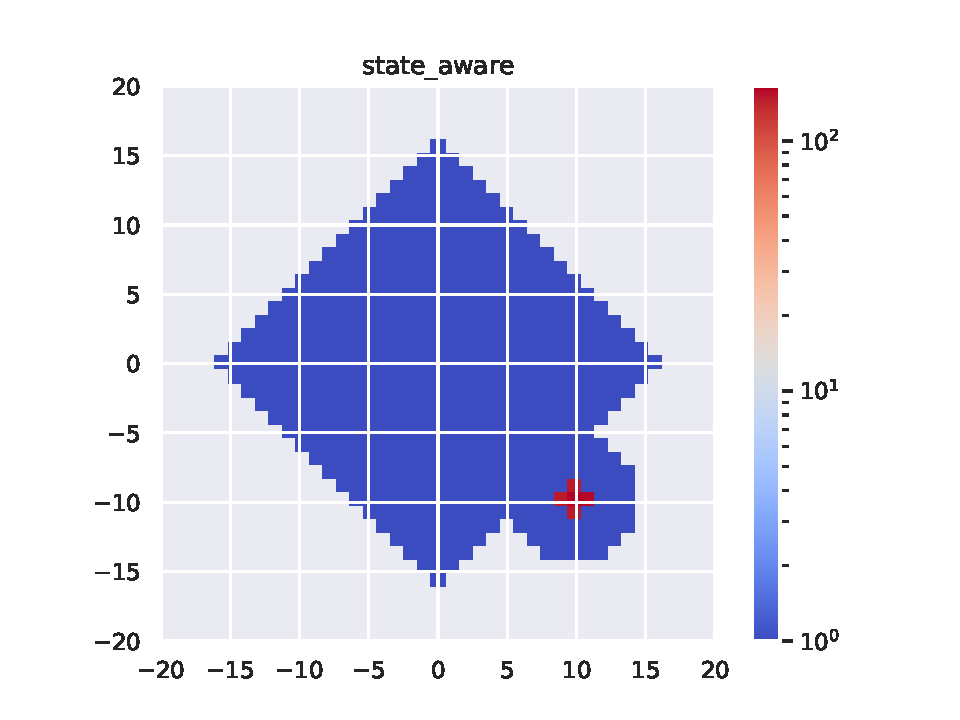
\includegraphics[width=0.49\linewidth]{img/epsilon/0/occupations_state_aware.pdf}
        \caption{$\epsilon=0$}
    \end{subfigure}
    \begin{subfigure}[b]{\textwidth}
        \centering
        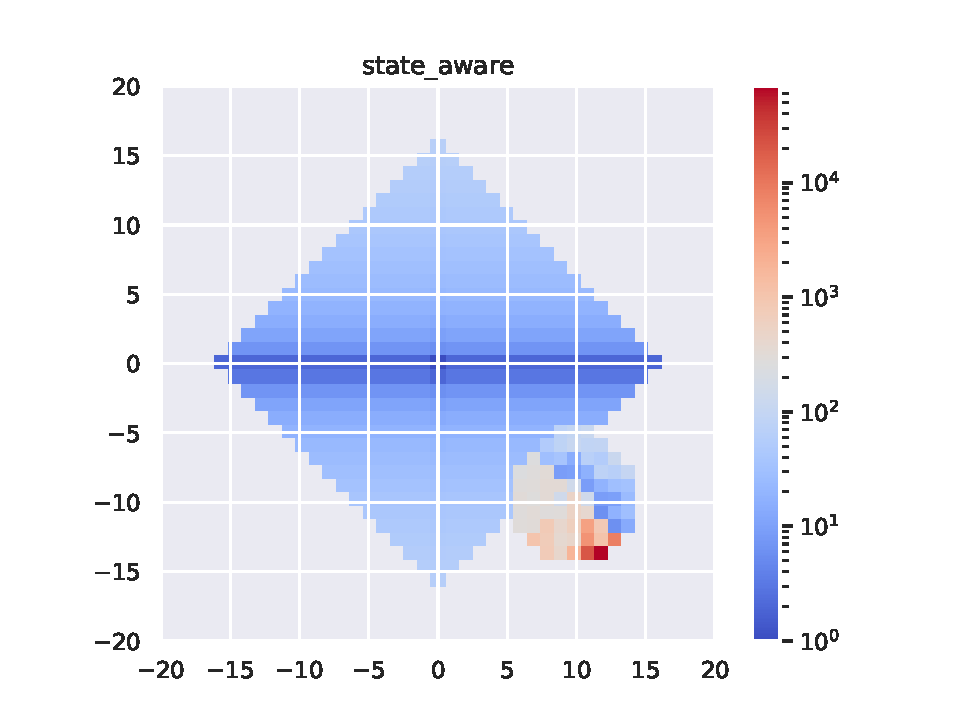
\includegraphics[width=0.49\textwidth]{img/epsilon/1e-2/updates_state_aware.pdf}
        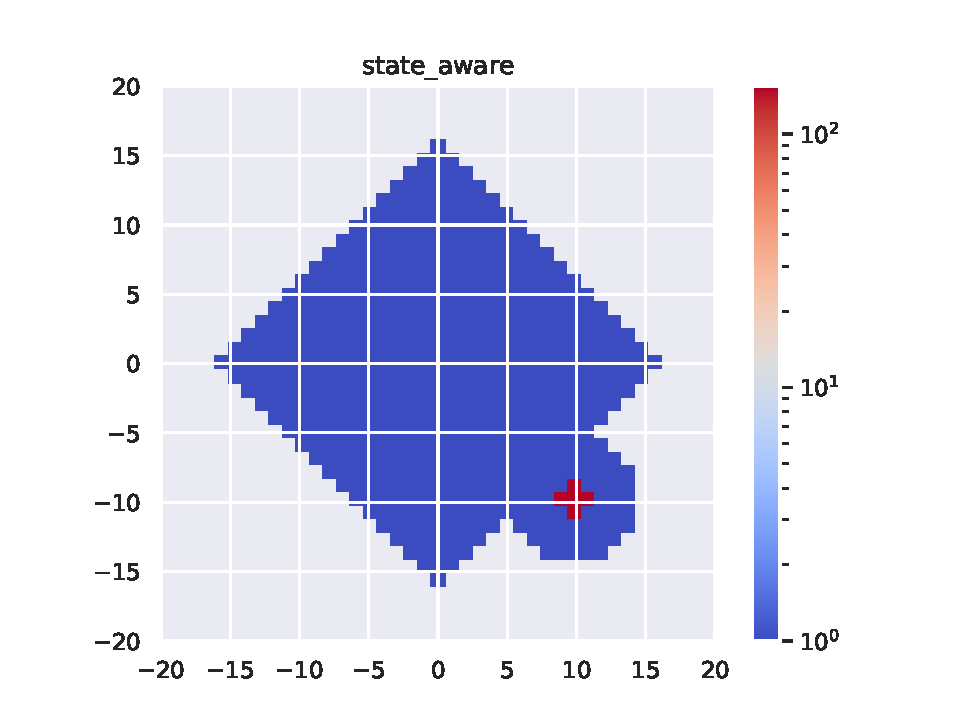
\includegraphics[width=0.49\textwidth]{img/epsilon/1e-2/occupations_state_aware.pdf}
        \caption{$\epsilon=1e-2$}
    \end{subfigure}
    \begin{subfigure}[b]{\textwidth}
        \centering
        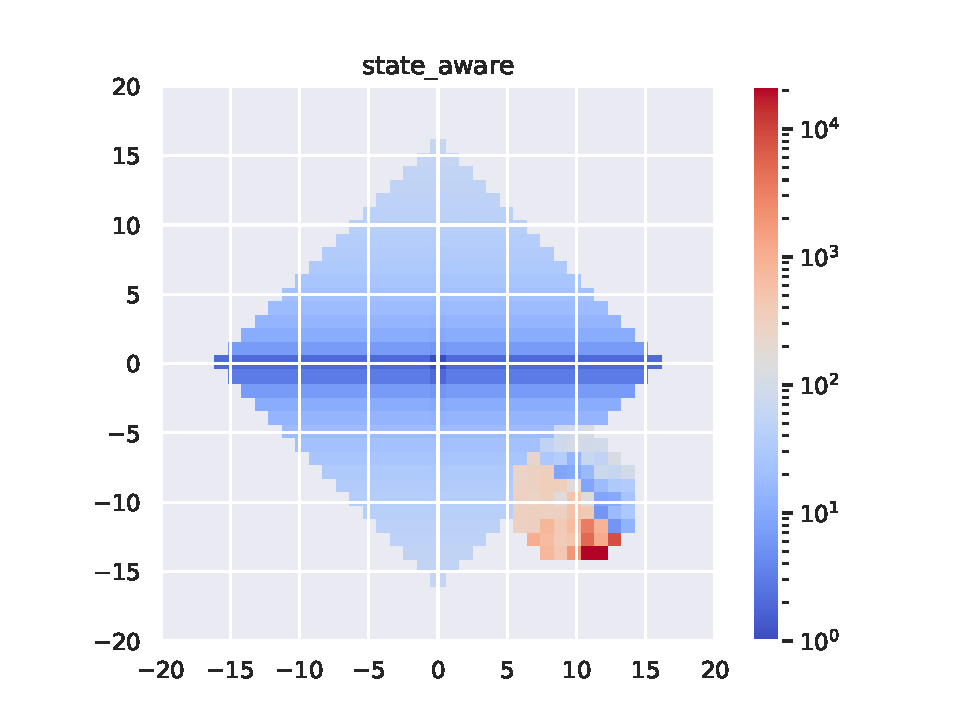
\includegraphics[width=0.49\textwidth]{img/epsilon/1e-1/updates_state_aware.pdf}
        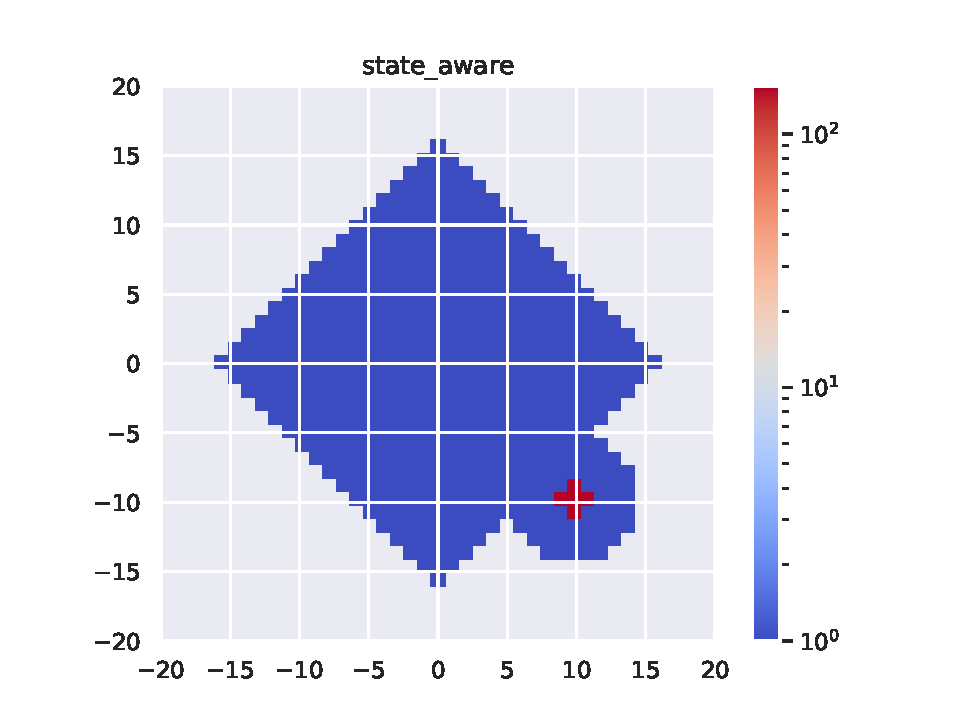
\includegraphics[width=0.49\textwidth]{img/epsilon/1e-2/occupations_state_aware.pdf}
        \caption{$\epsilon=1e-1$}
    \end{subfigure}
    \caption{Updates and occupancies for various values of $\epsilon$, for $n = 5460$, $\gamma=0.95$}
    \label{fig:epsilon_1}
\end{figure}
\begin{figure}[H]
\ContinuedFloat
    \centering
    \begin{subfigure}[b]{\textwidth}
        \centering
        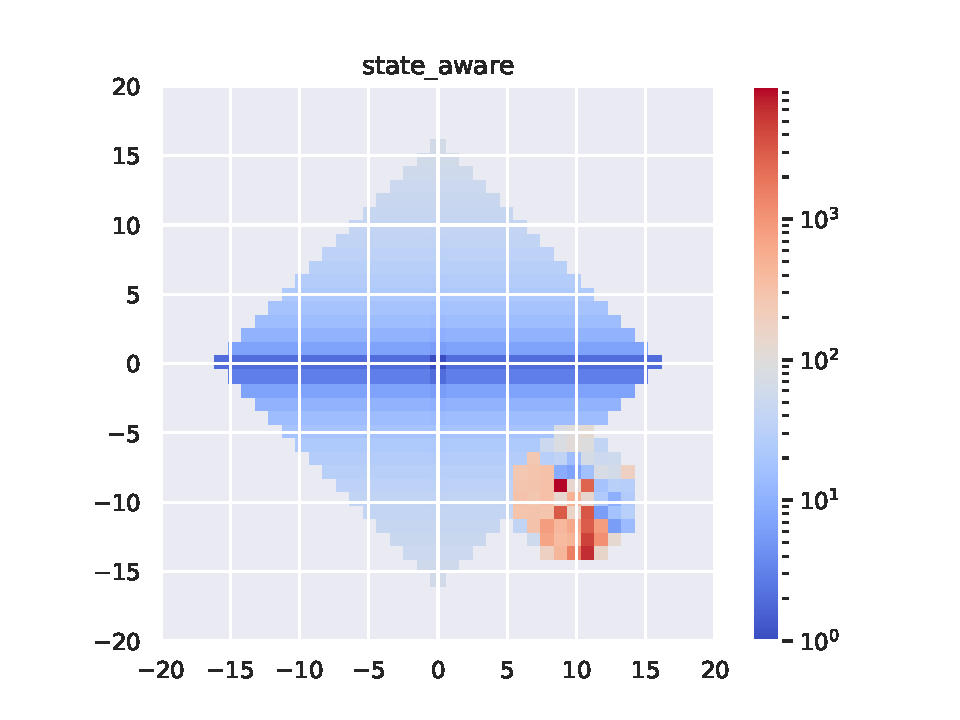
\includegraphics[width=0.49\textwidth]{img/epsilon/1e0/updates_state_aware.pdf}
        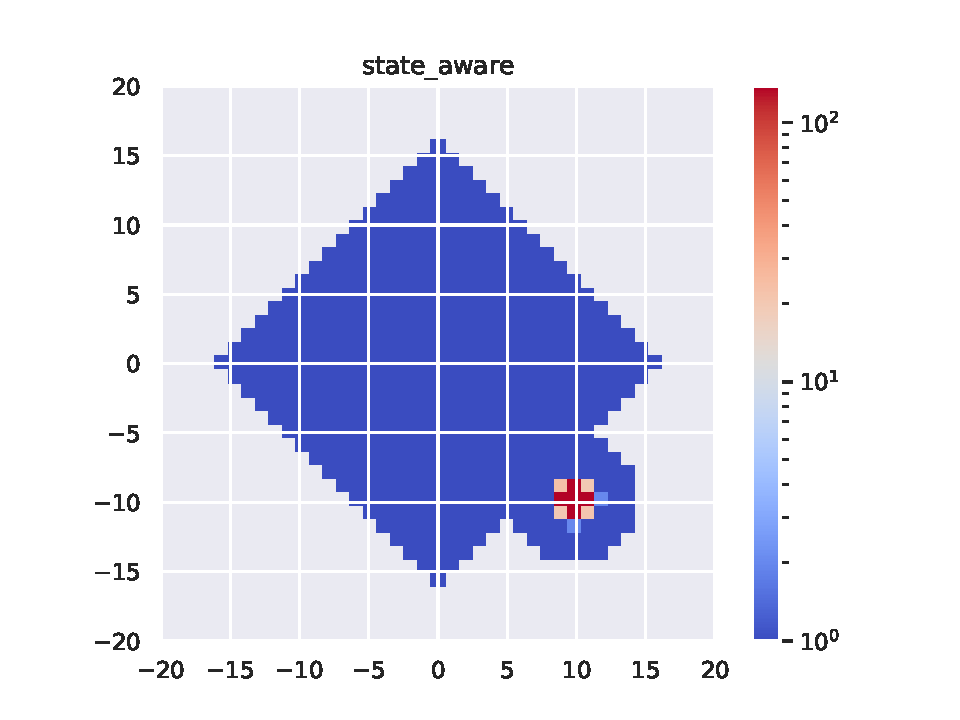
\includegraphics[width=0.49\textwidth]{img/epsilon/1e0/occupations_state_aware.pdf}
        \caption{$\epsilon=1e0$}
    \end{subfigure}
    \begin{subfigure}[b]{\textwidth}
        \centering
        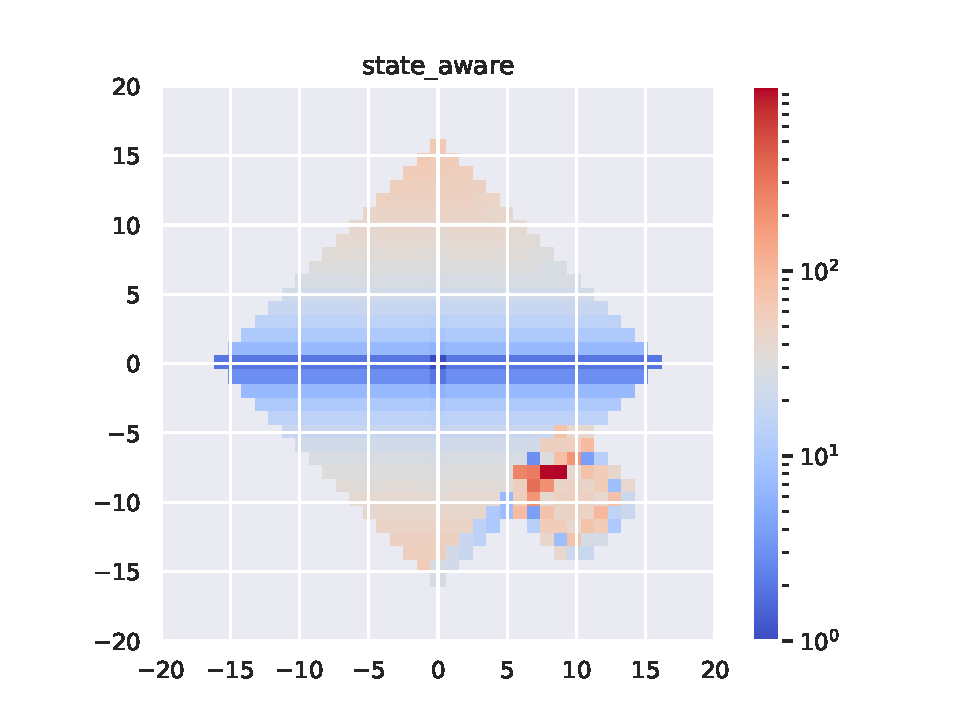
\includegraphics[width=0.49\textwidth]{img/epsilon/1e1/updates_state_aware.pdf}
        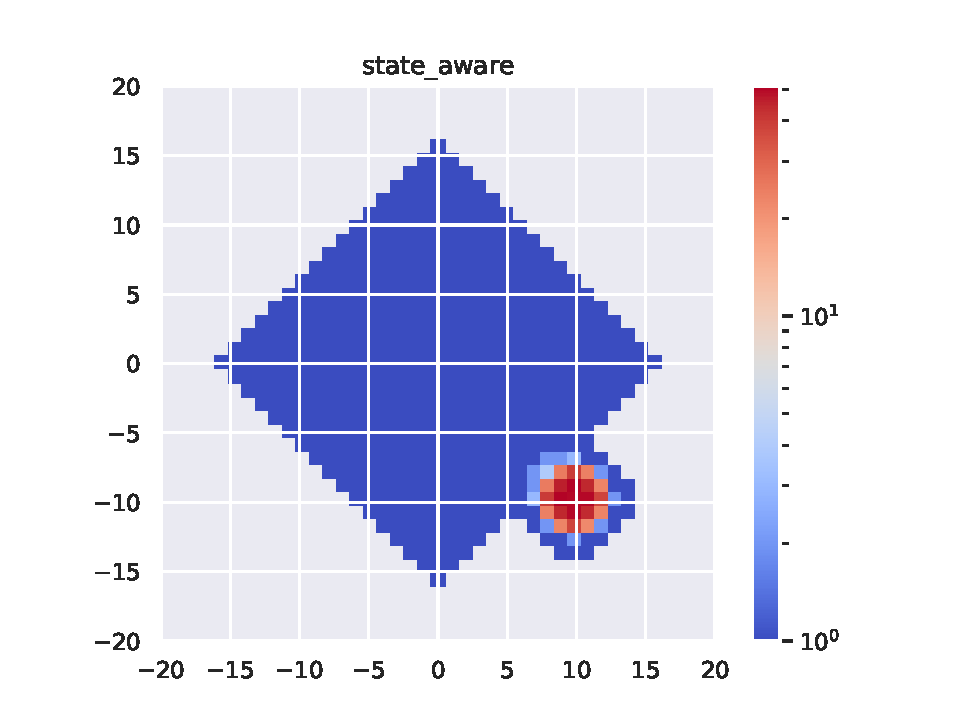
\includegraphics[width=0.49\textwidth]{img/epsilon/1e1/occupations_state_aware.pdf}
        \caption{$\epsilon=1e1$}
    \end{subfigure}
    \begin{subfigure}[b]{\textwidth}
        \centering
        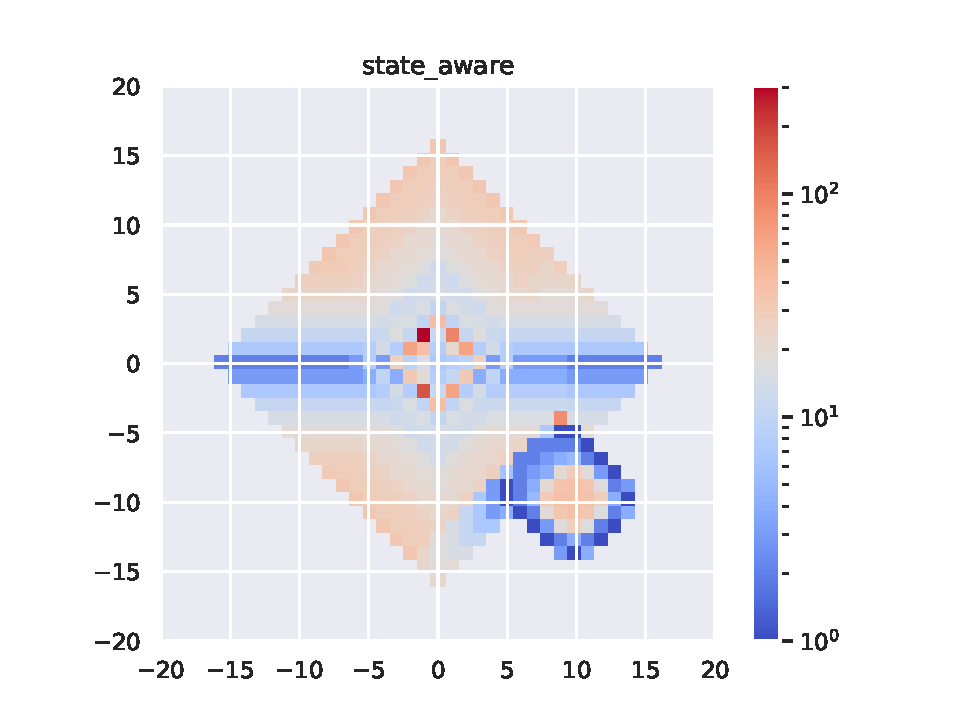
\includegraphics[width=0.49\textwidth]{img/epsilon/1e2/updates_state_aware.pdf}
        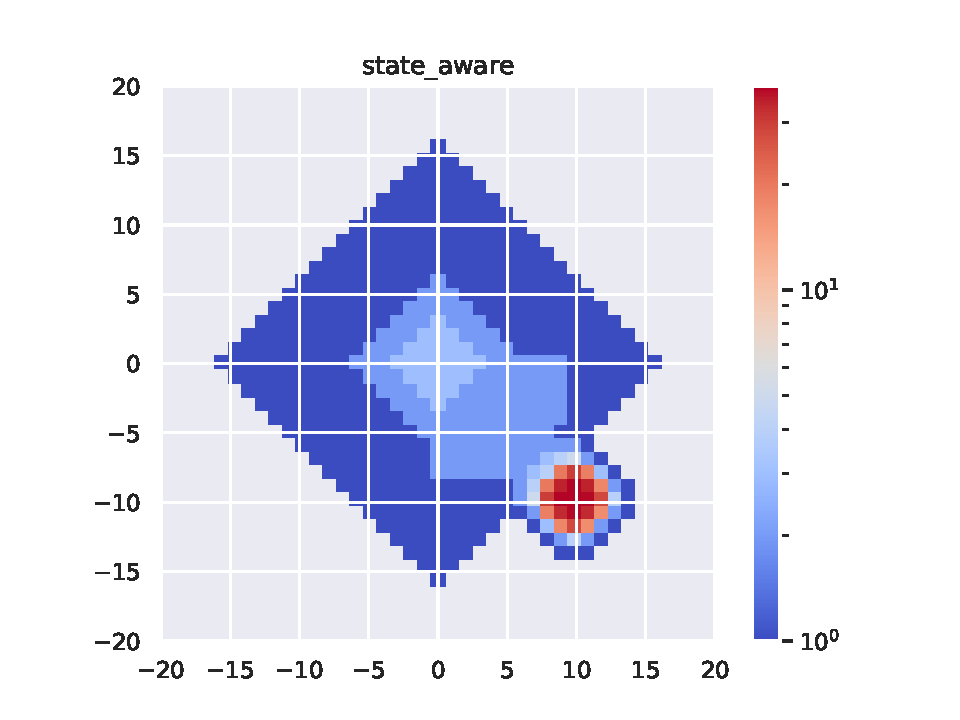
\includegraphics[width=0.49\textwidth]{img/epsilon/1e2/occupations_state_aware.pdf}
        \caption{$\epsilon=1e2 = V_{\max}$}
    \end{subfigure}
    \caption{Updates and occupancies for various values of $\epsilon$, for $n = 5460$, $\gamma=0.95$}
\end{figure}


\section{Extension to Stochastic MDPs}

If the transitions and rewards are stochastic, we can define 
state-aware upper/lower confidence bounds on the values in the following way. At each planning iteration,
\begin{enumerate}
    \item Make the graph of observed states and transitions $N(s), N(s,a), N(s,a,s'), R(s,a,s')$
    \item Unseen transitions $(s,a)$ go to the anonymous state $s_\emptyset$
    \item Estimate $r(s,a)$ and $p(s,a,s')$ based on previous observed samples
    \item Initialise $U_0 = V_{\max}, L_0 = 0$
    \item Backup each $(s,a)$ with $U_{k+1}(s) = \min(U_k(s), u(s,a) + \overline{p}_{s,a} U_k, U_k)$, until convergence (same resp. for $L$)
    \end{enumerate}
The memory complexity of iteration $n$ corresponds to maintaining a set of $n < |\mathcal{S}|$ state estimates and $nKB$ transitions. The planning algorithm then samples the next sequence based on the obtained intervals: start from the root and follow a BAI / Optimistic policy.

TODO: try on sailing env? or gridworld with noise: e.g. 0.5 chance of uneffective action. Plot the state occupancy: number of times a state was expanded ($N(s) > 1$)
    



\end{document}
